\label{chapt:intro}

Living in the era where it is nearly impossible to live without it, cellular service is very important. Up nearly 13\% from last year, it is said that US consumers are checking their mobile devices at a remarkable rate of 9 billion times per day \cite{deloittestat}.\\

It is numbers like these that have inspired \Company to begin research and development of the worlds first commercial, autonomous, aerostat's. Led by state of the art controls, Altaeros' mission is to help provide these services, including power in even the most remote of areas. The latest product is seen below in Figure~\ref{fig:1_companypic}~\cite{companypicweb}.

\begin{figure}[H]
    \centering
    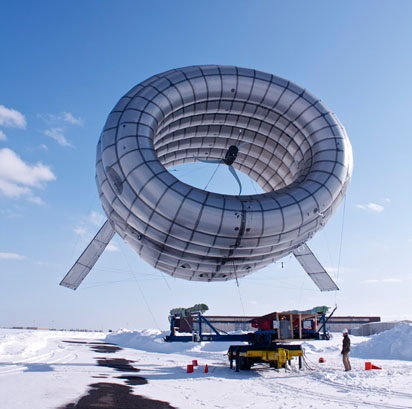
\includegraphics[width=0.6\textwidth]{1_companypic}
    \caption{Overview of the Altaeros' aerostat.}
    \label{fig:1_companypic}
\end{figure}


The above figure raises the question, how does this system remain stable. This is achieved through the system's tether management system.

\section{Background} % (fold)

Picture as per \cite{winchpic}.
\begin{figure}[H]
    \centering
    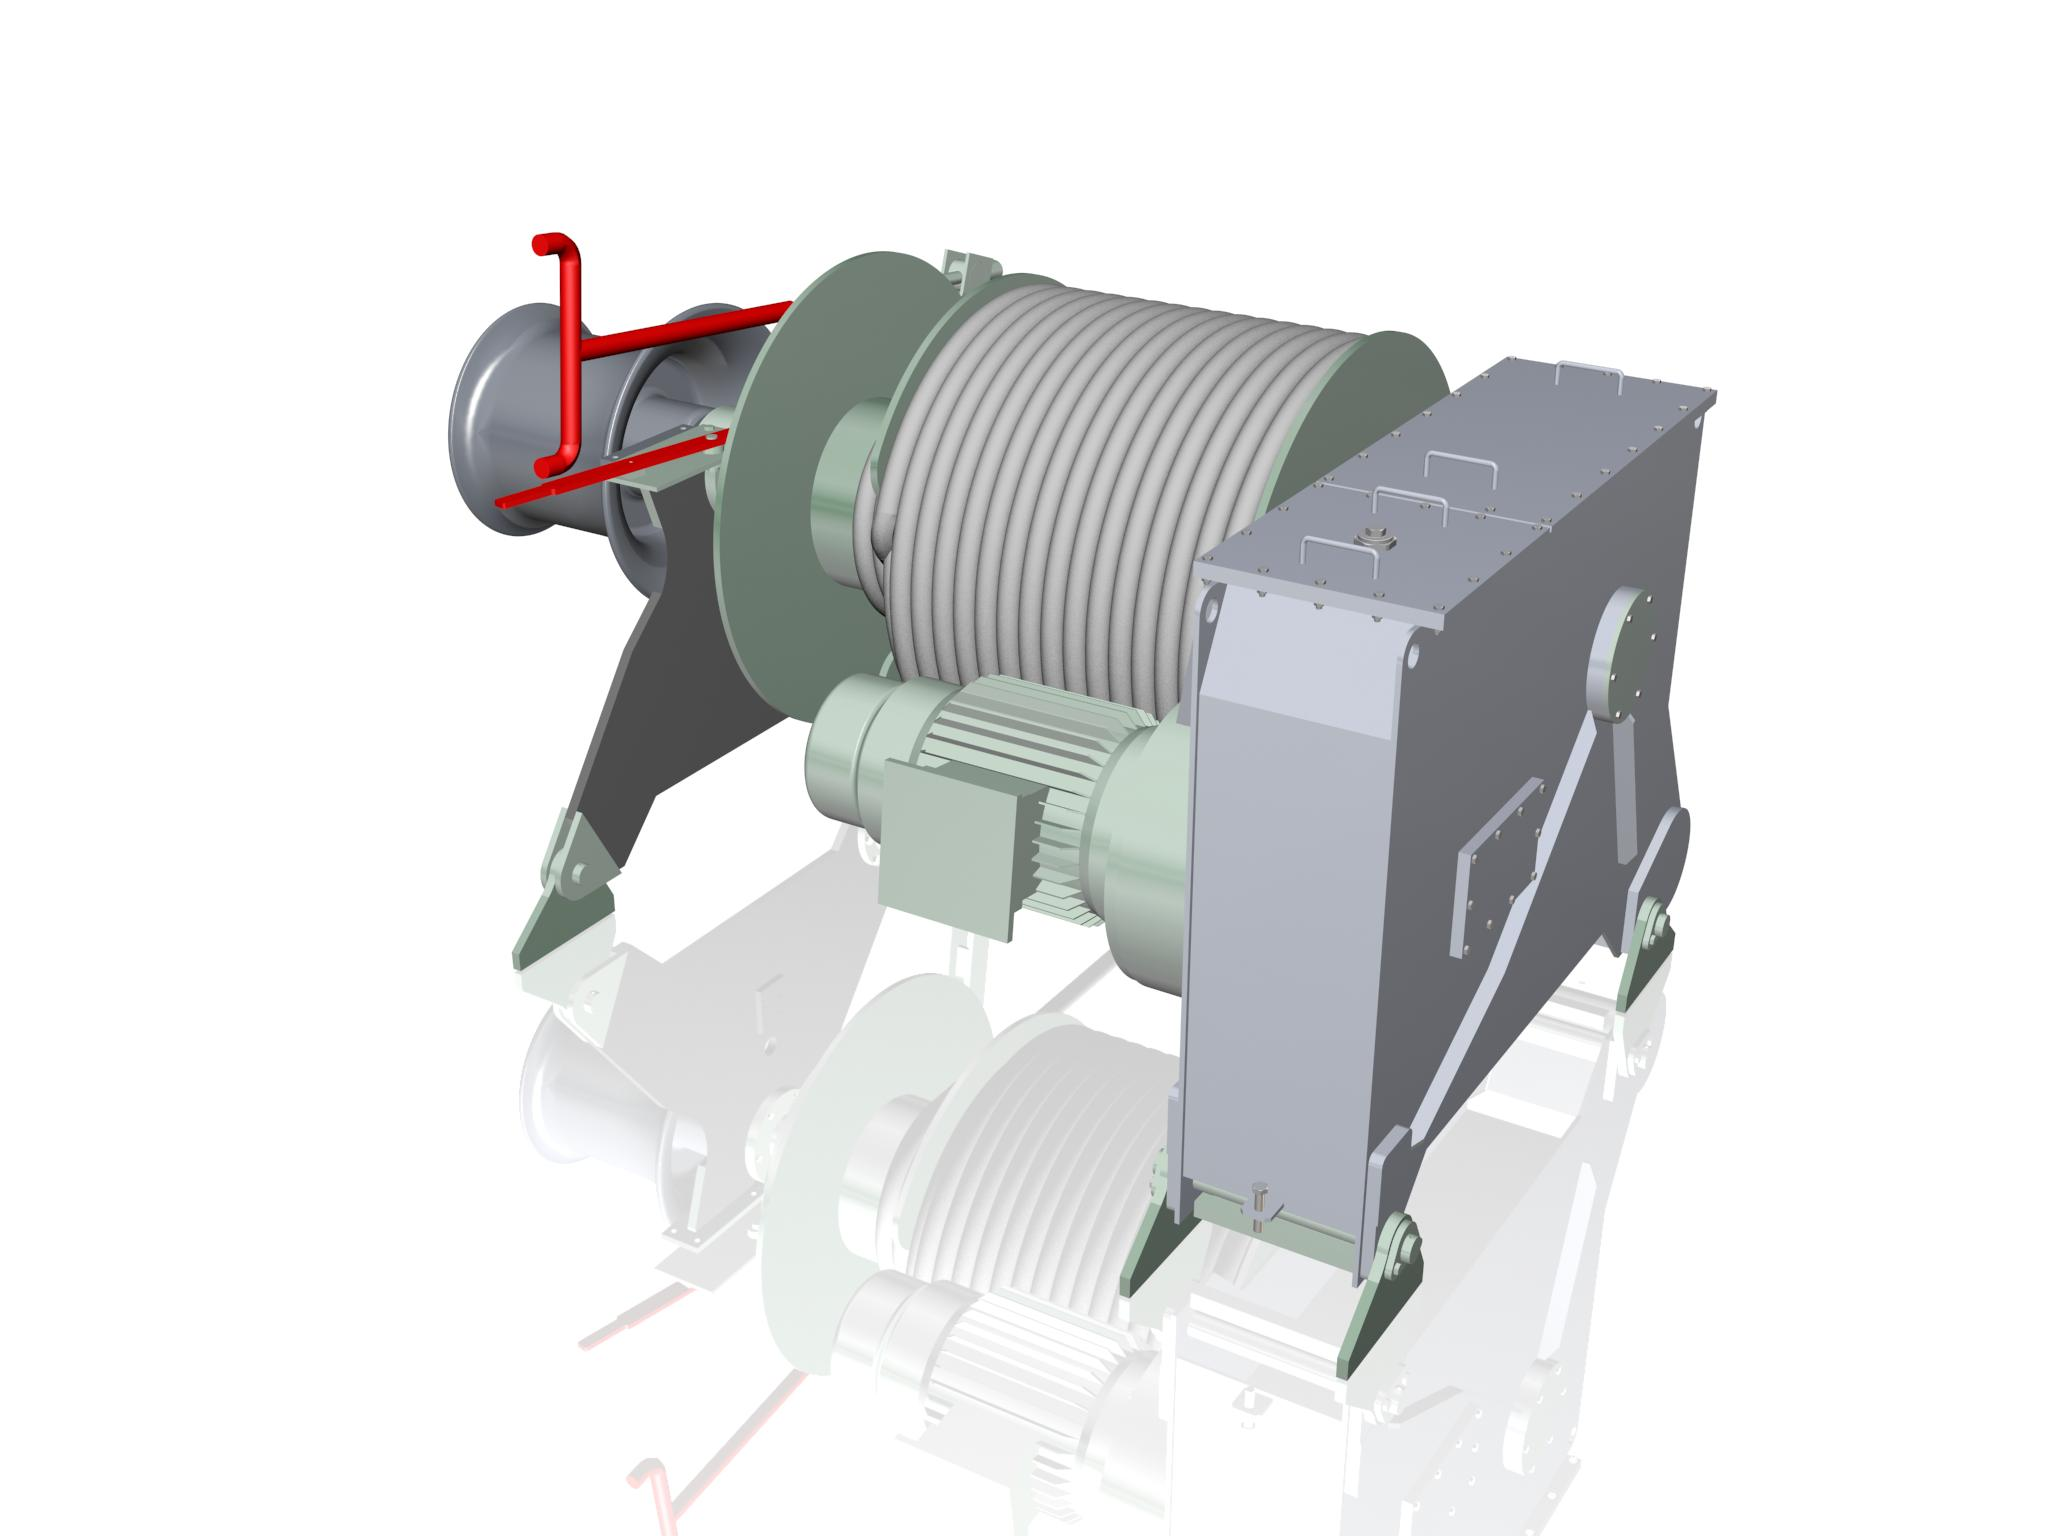
\includegraphics[width=0.6\textwidth]{1_winch}
    %% must use protect to put reference in caption
    \caption{Example of common winch system. \protect\cite{winchpic}}
    \label{fig:1_winch}
\end{figure}

\section{Purpose}
The purpose of this report is to do this.
\begin{itemize}
    \item Do analysis on drum
    \item Development numerical algorithm for solving
\end{itemize}


\section{Scope} % (fold)

The scope of the report will be as follows.
